\providecommand{\main}{../../..}
\documentclass[\main/main.tex]{subfiles}
\begin{document}

\subsection{Exercise 1}
Describe what is intended with the term \textit{preference relationship} in a complex decision problem.

Represent with a digraph the following preference relationship $\Pi$:

\begin{table}
  \begin{tabular}{L|LLLLL}
    \Pi   & f & f' & f'' & f''' & f'''' \\
    \hline
    f     & 1 & 0  & 1   & 1    & 1     \\
    f'    & 1 & 1  & 0   & 1    & 1     \\
    f''   & 0 & 0  & 1   & 1    & 1     \\
    f'''  & 0 & 0  & 0   & 1    & 0     \\
    f'''' & 0 & 0  & 1   & 0    & 1
  \end{tabular}
\end{table}

and build the \textit{incomparability relationship} associated to it.

Determine if the relationship $\Pi$ holds the reflexive, transitivity, antisymmetric and completeness property, specifying if it is an order relationship and if so, of which kind.

\subsection{Exercise 1 resolution}
A preference relationship $\Pi: D\rightarrow 2^{F\times F}$ is a binary relationship that associates to every decision maker a subset of tuples of impacts.

\begin{figure}
  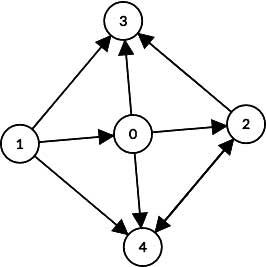
\includegraphics[width=0.3\textwidth]{20180124_01}
  \caption{Preference relationship oriented graph}
\end{figure}

\begin{description}
  \item[Reflexive property] The relationship \textit{holds} the reflexivity property as every impact is preferable to itself.
  \item[Transitive property] The relationship \textit{doesn't hold} the transitive property since the impact $f''''$ is preferable to the impact $f''$ and $f''$ is preferable to $f'''$, but $f'''' \not{\preceq} f'''$.
  \item[Antisymmetric property] The relationship \textit{doesn't hold} the antisymmetric property since the impact $f''$ and $f''''$ are interchangeable without being the same impact.
  \item[Completeness property] The relationship \textit{doesn't hold} the completeness property since the impact $f''''$ and $f'''$ have no preference relationship.
\end{description}

Every order relationship requires the transitive property, and this relationship doesn't hold it so it is not an order relationship.
\end{document}